\documentclass[aspectratio=169]{beamer}
\usepackage{color,amsmath}
\usepackage{subfigure}
\usepackage{booktabs}
\usepackage{framed}
\usepackage{comment}
\usepackage{hyperref}
\usepackage{ulem}

\usepackage{hyperref}
\hypersetup{
    colorlinks=true,
    linkcolor=blue,
    filecolor=magenta,      
    urlcolor=cyan,
}


%\usepackage{tikz}
%\beamertemplatenavigationsymbolsempty
%\usetikzlibrary{arrows,shapes.arrows,positioning,shapes}
%\newcommand\red[1]{{\color{red}#1}}
%\newcommand\bred[1]{{\color{red}\textbf{#1}}}
%\newcommand\blue[1]{{\color{blue}#1}}
%\newcommand\bblue[1]{{\color{blue}\textbf{#1}}}
%\newcommand\green[1]{{\color{olive}#1}}
%\newcommand\bgreen[1]{{\color{olive}\textbf{#1}}}
%\newcommand\black[1]{{\color{black}#1}}
%\newcommand\white[1]{{\color{white}#1}}
%\newcommand\E{\text{E}}
%\newcommand\V{\text{V}}
%\renewcommand\P{\text{P}}


\title{Participating in the Fragile Families Challenge Activity}
\author{{\small Matthew Salganik, Ian Lundberg, Alex Kindel, Sara McLanahan,\\and people from around the world}}
\date[]{
\begin{flushleft}{\tiny Funding for FFCWS provided by NICHD (R01HD36916, R01HD39135, R01HD40421) and a consortium of private foundations, including the Robert Wood Johnson Foundation. Funding for FFC provided by the Russell Sage Foundation, NSF, \& the Overdeck Fund. FFC Board of Advisors: Jeanne Brooks-Gunn, Kathryn Edin, Barbara Engelhardt, Irwin Garfinkel, Moritz Hardt, Dean Knox, Nicholas Lemann, Karen Levy, Sara McLanahan, Arvind Narayanan, Timothy Nelson, Matthew Salganik, Brandon Stewart \& Duncan Watts.}
\end{flushleft}
\begin{flushright}

\includegraphics[width=0.1\textwidth]{figures/cc-by.png}
\end{flushright}
}

\begin{document}
%%%%%%%%%%%%%%%%%%%%%%%%%%
\frame{\titlepage}
%%%%%%%%%%%%%%%%%%%%%%%%%%%
\begin{frame}

\begin{center}
\includegraphics[width=\textwidth]{figures/ffc_design_matrix_ml}
\end{center}

\end{frame}
%%%%%%%%%%%%%%%%%%%%%%%%%
\begin{frame}

\Large{
\begin{center}
Introducing the outcome variables
\end{center}
}

\end{frame}
%%%%%%%%%%%%%%%%%%%%%%%%%
\begin{frame}

\Large{
\begin{center}
GPA\footnote{Learn more at \url{http://www.fragilefamilieschallenge.org/gpa/}}
\end{center}
}

\end{frame}
%%%%%%%%%%%%%%%%%%%%%%%%%
\begin{frame}{GPA\footnote{This variable is reverse-coded in the data file so that higher values represent higher GPAs.}}

\centering
\includegraphics[width = .9\textwidth]{figures/GPA_questionnaire}

\end{frame}
%%%%%%%%%%%%%%%%%%%%%%%%%
\begin{frame}

\centering
\includegraphics[width = .8\textwidth]{figures/gpaDist}

\end{frame}

%%%%%%%%%%%%%%%%%%%%%%%%%
\begin{frame}

\Large{
\begin{center}
Grit\footnote{Learn more at \url{http://www.fragilefamilieschallenge.org/grit/}} 
\end{center}
}

\end{frame}
%%%%%%%%%%%%%%%%%%%%%%%%%%%
\begin{frame}{Grit\footnote{This variable is reverse-coded in the data file so that higher values represent more grit.}}

\centering
\includegraphics[width = .9\textwidth]{figures/grit_questionnaire2}

\end{frame}
%%%%%%%%%%%%%%%%%%%%%%%%%
\begin{frame}

\centering
\includegraphics[width = .8\textwidth]{figures/gritDist}

\end{frame}
%%%%%%%%%%%%%%%%%%%%%%%%%

\begin{frame}

\Large{
\begin{center}
Material hardship\footnote{Learn more at \url{http://www.fragilefamilieschallenge.org/material-hardship/}} 
\end{center}
}

\end{frame}
%%%%%%%%%%%%%%%%%%%%%%%%%%%
\begin{frame}{Material hardship}

\centering
\includegraphics[width = .9\textwidth]{figures/materialHardship_questionnaireA}

\end{frame}
%%%%%%%%%%%%%%%%%%%%%%%%%%%
\begin{frame}{Material hardship}

\centering
\includegraphics[width = .9\textwidth]{figures/materialHardship_questionnaireB}

\end{frame}
%%%%%%%%%%%%%%%%%%%%%%%%%
\begin{frame}

\centering
\includegraphics[width = .8\textwidth]{figures/materialHardshipDist}

\end{frame}
%%%%%%%%%%%%%%%%%%%%%%%%%
\begin{frame}

\Large{
\begin{center}
Eviction\footnote{Learn more at \url{http://www.fragilefamilieschallenge.org/eviction/}}
\end{center}
}

\end{frame}
%%%%%%%%%%%%%%%%%%%%%%%%%%%
\begin{frame}{Eviction}

\centering
\includegraphics[width = .9\textwidth]{figures/eviction_questionnaire}

\end{frame}
%%%%%%%%%%%%%%%%%%%%%%%%%
\begin{frame}

\centering
\includegraphics[width = .8\textwidth]{figures/evictionDist}

\end{frame}
%%%%%%%%%%%%%%%%%%%%%%%%%
\begin{frame}

\Large{
\begin{center}
Caregiver layoff\footnote{Learn more at \url{http://www.fragilefamilieschallenge.org/layoff/}\vskip .2cm}
\end{center}
}

\end{frame}
%%%%%%%%%%%%%%%%%%%%%%%%%%%
\begin{frame}{Caregiver layoff}

\centering
\includegraphics[width = .9\textwidth]{figures/layoff_questionnaire}

\end{frame}
%%%%%%%%%%%%%%%%%%%%%%%%%
\begin{frame}

\centering
\includegraphics[width = .8\textwidth]{figures/layoffDist}

\end{frame}
%%%%%%%%%%%%%%%%%%%%%%%%%
\begin{frame}

\Large{
\begin{center}
Job training\footnote{Learn more at \url{http://www.fragilefamilieschallenge.org/job-training/}\vskip .2cm}
\end{center}
}

\end{frame}
%%%%%%%%%%%%%%%%%%%%%%%%%%%
\begin{frame}{Caregiver job training}

\centering
\includegraphics[width = .9\textwidth]{figures/jobTraining_questionnaire}

\end{frame}
%%%%%%%%%%%%%%%%%%%%%%%%%
\begin{frame}

\centering
\includegraphics[width = .8\textwidth]{figures/jobTrainingDist}

\end{frame}
%%%%%%%%%%%%%%%%%%%%%%%%%%%
\begin{frame}

\begin{enumerate}
\item Prepare data
\item Create predictive model
\item Upload submission
\end{enumerate}

\end{frame}
%%%%%%%%%%%%%%%%%%%%%%%%%
\begin{frame}

\begin{enumerate}
\item \textcolor{blue}{Prepare data}
\item Create predictive model
\item Upload submission
\end{enumerate}

\end{frame}
%%%%%%%%%%%%%%%%%%%%%%%%%
\begin{frame}

\textbf{The Fragile Families and Child Wellbeing Study is a dataset of real people who have selflessly opened up their lives to us for the last 15 years so that their experiences can contribute to scientific research. By participating in the Fragile Families Challenge activity, you become a collaborator in this project. It is of the utmost importance that you respect the families in the data by using what they have told us responsibly.}

\end{frame}
%%%%%%%%%%%%%%%%%%%%%%%%%
\begin{frame}

\begin{itemize}
\item When you applied to get access to the data, you completed a data use agreement. Honor that agreement.
\pause
\item After this activity you should delete the data from your computer. If you plan to do more research, you can download it again.
\end{itemize}

\end{frame}
%%%%%%%%%%%%%%%%%%%%%%%%
\begin{frame}

\begin{center}
\includegraphics[width=0.8\textwidth]{figures/ff_design_public2}
\end{center}

\end{frame}
%%%%%%%%%%%%%%%%%%%%%%%%%
\begin{frame}

\begin{center}
\includegraphics[width=\textwidth]{figures/ffc_rawdata_f5f}
\end{center}

\end{frame}
%%%%%%%%%%%%%%%%%%%%%%%%%
%\begin{frame}
%
%\begin{center}
%\includegraphics[width=\textwidth]{figures/scientific_pipeline}
%\end{center}
%
%\end{frame}
%%%%%%%%%%%%%%%%%%%%%%%%%%
%\begin{frame}
%
%\begin{itemize}
%\item A team of people\footnote{Alexander Kindel, Vineet Bansal, Kristin Catena, Thomas Hartshorne, Kate Jaeger, Dawn Koffman, Sara McLanahan, Maya Phillips, Shiva Rouhani, Ryan Vinh, Matthew Salganik.} has spent months making the data easier to use. \pause
%\item Is it possible to do better than last time? Or, is there a fundamental limit with this data and this task? \pause
%\item Let's see if it improves performance, \pause and let's see if you can help make this easier for future researchers.
%\end{itemize}
%
%\end{frame}
%%%%%%%%%%%%%%%%%%%%%%%%%%
\begin{frame}

How do I know what these variables are? 

\end{frame}
%%%%%%%%%%%%%%%%%%%%%%%%
\begin{frame}

\centering\includegraphics[width = .8\textwidth]{figures/Doc1}

\end{frame}
%%%%%%%%%%%%%%%%%%%%%%%%%%%
\begin{frame}

\centering\includegraphics[width = .8\textwidth]{figures/Doc2}

\end{frame}
%%%%%%%%%%%%%%%%%%%%%%%%%%%
\begin{frame}

\centering\includegraphics[width = .8\textwidth]{figures/Doc3}

\end{frame}
%%%%%%%%%%%%%%%%%%%%%%%%%%%
\begin{frame}

Questionnaire:\\
\centering\includegraphics[width = .8\textwidth]{figures/f5f1_skip}

\end{frame}
%%%%%%%%%%%%%%%%%%%%%%%%%%
\begin{frame}

\begin{center}
\includegraphics[width=0.95\textwidth]{figures/frustrating}
\end{center}

\vfill
\tiny{\url{https://www.talk2solicitors.co.uk/blog/limits-frustration-contract/}}

\end{frame}
%%%%%%%%%%%%%%%%%%%%%%%%%%%%
\begin{frame}

\begin{center}
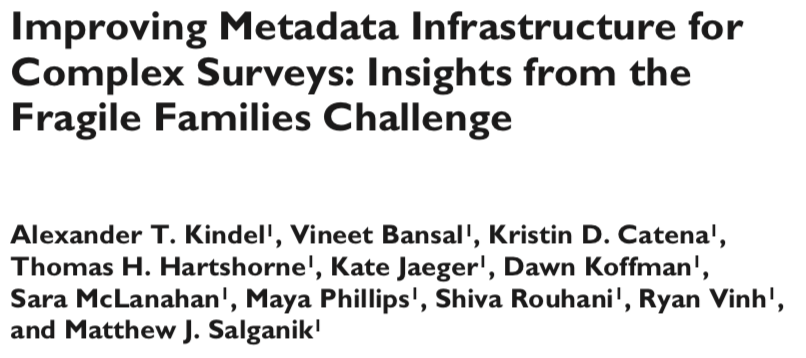
\includegraphics[width=0.95\textwidth]{figures/kindel_improving_2019_title}
\end{center}

\vfill
\href{https://doi.org/10.1177/2378023118817378}{Kindel et al.\ (2019)}
\end{frame}
%%%%%%%%%%%%%%%%%%%%%%%%%%%%
\begin{frame}

\begin{center}
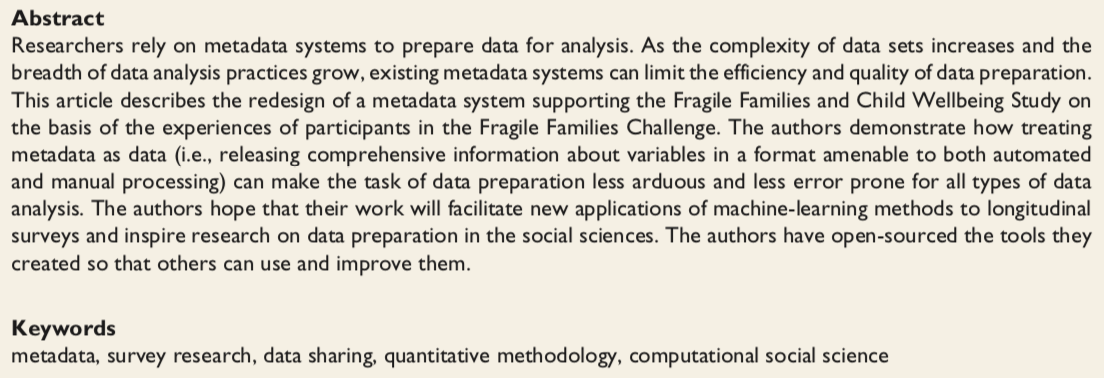
\includegraphics[width=0.95\textwidth]{figures/kindel_improving_2019_abs}
\end{center}

\vfill
\href{https://doi.org/10.1177/2378023118817378}{Kindel et al.\ (2019)}
\end{frame}
%%%%%%%%%%%%%%%%%%%%%%%%%%%%
\begin{frame}

\begin{itemize}
\item Data preparation is a barrier to progress in predictive modeling in the social sciences.
\pause
\item New approach to metadata: Human-readable $\rightarrow$ machine-actionable.
\end{itemize}

\vfill
\href{https://doi.org/10.1177/2378023118817378}{Kindel et al.\ (2019)}

\end{frame}
%%%%%%%%%%%%%%%%%%%%%%%%%%%%
\begin{frame}

How do I know what these variables are? 

\begin{center}
\includegraphics[width=0.7\textwidth]{figures/ff_metadata_browser}
\end{center}

\vfill

\url{http://metadata.fragilefamilies.princeton.edu/variables}

\end{frame}
%%%%%%%%%%%%%%%%%%%%%%%%%%%
\begin{frame}

Introducing \texttt{cm1relf}\\

\url{http://metadata.fragilefamilies.princeton.edu/variables/cm1relf}

\end{frame}
%%%%%%%%%%%%%%%%%%%%%%%%%%%
\begin{frame}

You can filter variables by:
\begin{itemize}
\item Topic
\item Wave
\item Respondent
\item Variable Type (e.g., continuous, ordered categorical, unordered categorical, etc).
\end{itemize}

\end{frame}	
%%%%%%%%%%%%%%%%%%%%%%%%%%%
\begin{frame}

Direct access to the metadata:
\begin{itemize}
\item API: \url{api.metadata.fragilefamilies.princeton.edu}
\item Python package: \url{github.com/fragilefamilieschallenge/ffmetadata-py}
\item R package: \url{github.com/fragilefamilieschallenge/ffmetadata}
\item Raw metadata: \url{api.fragilefamiliesmetadata.org/get_metadata}
\end{itemize}

\end{frame}
%%%%%%%%%%%%%%%%%%%%%%%%%%%
\begin{frame}

Why \texttt{cm1relf}? \pause

\begin{center}
\includegraphics[width=\textwidth]{figures/ff_variablename_standards}
\end{center}

\end{frame}
%%%%%%%%%%%%%%%%%%%%%%%%%%
\begin{frame}

Advice for data preparation
\begin{itemize}
\item do something about missing data
\item do something about unordered categorical variables
\end{itemize}

\end{frame}
%%%%%%%%%%%%%%%%%%%%%%%%%%
\begin{frame}
\frametitle{Advice for data preparation}

Deal with missing data

\begin{center}
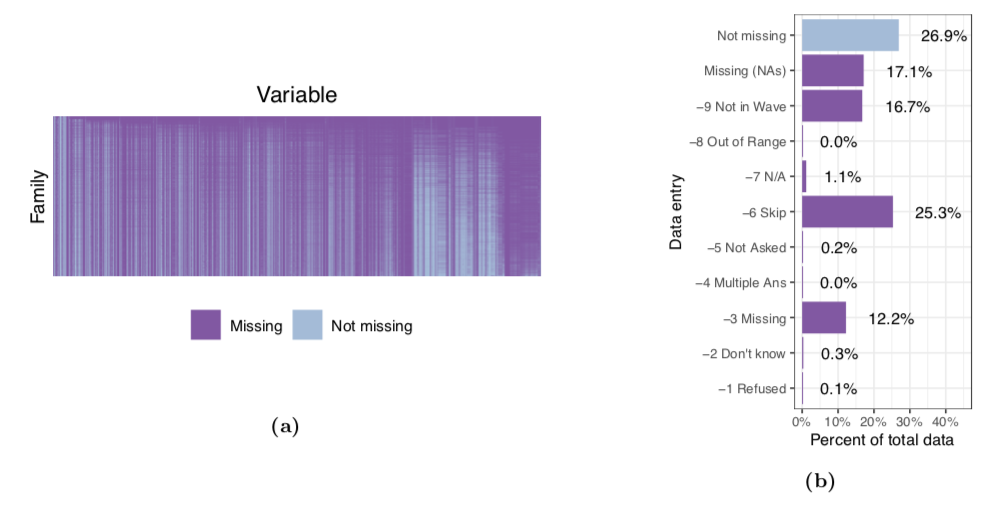
\includegraphics[width = \textwidth]{figures/salganik_measuring_2020_figs1}
\end{center}

\vfill
Given that we have only a few hours, I would recommend not worrying about this too much.  In the \href{https://journals.sagepub.com/topic/collections-srd/srd-1-fragile_families/srd}{\textit{Socius} Special Collection}, we saw some evidence that complex approaches to missing data didn't help much.
\end{frame}
%%%%%%%%%%%%%%%%%%%%%%%%%%%
\begin{frame}
\frametitle{Advice for data preparation}

Deal with unordered categorical variables

\begin{center}
\includegraphics[width=0.8\textwidth]{figures/f5f3b1}
\end{center}

\end{frame}
%%%%%%%%%%%%%%%%%%%%%%%%%%%%
\begin{frame}

\begin{enumerate}
\item \textcolor{blue}{Prepare data}
\item Create predictive model
\item Upload submission
\end{enumerate}

\end{frame}
%%%%%%%%%%%%%%%%%%%%%%%%%
\begin{frame}

\begin{enumerate}
\item Prepare data
\item \textcolor{blue}{Create predictive model}
\item Upload submission
\end{enumerate}

\end{frame}
%%%%%%%%%%%%%%%%%%%%%%%%%
\begin{frame}
Here are some approaches that participants used in the Challenge (key ideas are flexibility and over-fitting):

\begin{itemize}
\item general linear model (linear and logistic regression)
\item Tree-based methods (e.g., random forrest, gradient boosted trees)
\item Regularization approaches (e.g., LASSO, Ridge, Elastic Net)
\end{itemize}

\end{frame}
%%%%%%%%%%%%%%%%%%%%%%%%%
\begin{frame}

\begin{enumerate}
\item Prepare data
\item \textcolor{blue}{Create predictive model}
\item Upload submission
\end{enumerate}

\end{frame}
%%%%%%%%%%%%%%%%%%%%%%%%%
\begin{frame}

\begin{enumerate}
\item Prepare data
\item Create predictive model
\item \textcolor{blue}{Upload submission}
\end{enumerate}

\end{frame}
%%%%%%%%%%%%%%%%%%%%%%%%%
\begin{frame}
\frametitle{Building a submission}

Submissions include:
\begin{enumerate}
\item Predictions
\item Code
\item Narrative explanation
\end{enumerate}

\vfill
See the \href{https://github.com/compsocialscience/summer-institute/blob/master/2020/materials/day5-mass-collaboration/activity/lesson_plan_masscollaboration_participant.md}{lesson plan for participants} for more information about building and uploading your submission

\end{frame}
%%%%%%%%%%%%%%%%%%%%%%%%%%%
\begin{frame}{Get on the leaderboard}

\includegraphics[width = 0.9\textwidth]{figures/leaderboard}

\end{frame}
%%%%%%%%%%%%%%%%%%%%%%%%%%%
\begin{frame}

\begin{enumerate}
\item Prepare data
\item Create predictive model
\item Upload submission
\end{enumerate}

\end{frame}
%%%%%%%%%%%%%%%%%%%%%%%%%%%
\begin{frame}

\begin{center}
\LARGE Remember this is not easy,\\ especially in a short amount of time.
\end{center}

\end{frame}
%%%%%%%%%%%%%%%%%%%%%%%%%%%%%%%
\begin{frame}

\begin{center}
\LARGE Good luck and enjoy
\end{center}

\end{frame}
%%%%%%%%%%%%%%%%%%%%%%%%%%%%%%%

\end{document}